\documentclass[a4paper,12pt]{article}
\usepackage{amsmath, amsfonts, amssymb,  textcomp, amsthm, multicol}
\usepackage[T1, T2A]{fontenc}
\usepackage[utf8]{inputenc}
\usepackage[english, russian]{babel}
\usepackage[nottoc,numbib]{tocbibind}
\usepackage{mathtext}
\usepackage{hyperref}
\usepackage{enumitem}
\usepackage{graphicx}
\usepackage{extsizes}

\usepackage{minted}

\usepackage[
    backend=biber%,
%    style=authoryear-icomp,
%    sortlocale=de_DE,
%    natbib=true,
%    url=false, 
%    doi=true,
%    eprint=false
]{biblatex}
\addbibresource{literature.bib}

\begin{document}
\renewcommand{\sfdefault}{ptm}

\newcommand{\sumfromto}[3]{\overset{#2}{\underset{#1}{\sum}}{#3}}

\begin{titlepage}

\newcommand{\HRule}{\rule{\linewidth}{0.5mm}} % Defines a new command for the horizontal lines, change thickness here

\center 


\Large Московский государственный университет имени М.В. Ломоносова\\[1.5cm]
\Large Факультет вычислительной математики и кибернетики\\[0.5cm]
\large Реферат\\[0.5cm] 

%\HRule \\[0.4cm]
{ \huge \bfseries Метод натурального градиента}\\[0.4cm] % Title of your document
%\HRule \\[1.5cm]

\begin{flushright} \large
\Large \emph{Исполнитель:}\\
Виктор Януш\\[3cm] 
\end{flushright}

\vfill 

{\large Москва \\ 2016 год}\\[3cm]
%{\large \today}\\[3cm] % Date, change the \today to a set date if you want to be precise

\end{titlepage}

%\maketitle
 
\tableofcontents
\newpage

%\addcontentsline{toc}{section}{Unnumbered Section}

\section{Введение}

Стандартный метод градиентного спуска является часто используемым методом оптимизации функций,
однако он не всегда сходится быстро и зависит от того пространства, в котором находятся параметры
оптимизируемой функции. В этом реферате рассматривается метод натурального градиента, который иногда 
позволяет обойти эти ограничения, используя внутреннюю риманову структуру пространства параметров. 
В частности, для задачи оптимизации функции максимального правдоподобия метод натурального градиента 
является асимптотически эффективным по Фишеру \cite{AmariWorks}.

\newpage 

\section{Градиентный спуск}
Предположим, что перед нами стоит задача минимизировать некоторую функцию $f(x) : \mathbb{R}^{n} \rightarrow \mathbb{R}$. \\
Рассмотрим линейное приближение $f(x)$ в точке $x_0$ при достаточно малом $||x - x_0||$:
$$f(x) \approx f(x_0) + \nabla{f(x_0)}^{T}(x - x_0)$$
Пусть $x - x_0 = \alpha \widetilde{d} $, где $||\widetilde{d}|| = 1, ~ \alpha > 0$.  \\ 
Ясно, что:
$$\underset{\widetilde{d}}{argmin} f(x) \approx 
\underset{\widetilde{d}}{argmin} (f(x_0) + \alpha \nabla{f(x_0)}^{T}\widetilde{d}) = 
\underset{\widetilde{d}}{argmin} \nabla{f(x_0)}^{T}\widetilde{d} = 
-\frac{\nabla{f(x_0)}}{||\nabla{f(x_0)}||}$$

\noindent Таким образом, направлением наискорейшего спуска является:
$$\widetilde{d} = -\frac{\nabla{f(x_0)}}{||\nabla{f(x_0)}||}$$
Приходим к следующему алгоритму градиентного спуска:
\begin{enumerate}
    \item Выбираем $x_0, \varepsilon $ и инициализируем $k \leftarrow 0$
    \item $d_k = -\nabla{f(x_k)}$.
    \item Если $||d_k|| < \varepsilon$, то выход.
    \item $x_{k+1} \leftarrow x_{k} + \alpha_k d_k, ~ k \leftarrow k + 1$. Переход к шагу 2. 
\end{enumerate}

Проблема этого метода заключается в том, что он зависит от системы координат. К примеру, если
мы перейдем к $y: x = Ay$, то получится следующая формула: \\
$$y_{k+1} = y_{k} - \alpha_k \nabla_y{f(Ay)} = y_{k} - \alpha_k A^T \nabla_x{f(Ay)}$$
$$Ay_{k+1} = Ay_{k} - \alpha_k AA^T \nabla_x{f(Ay)}$$
Проблема в том, что $Ay_{k+1} \neq x_{k+1}$ \\

Отсюда следует, что, вообще говоря, скорость сходимости метода может зависеть от системы координат. \\

\newpage


\section{Метод Ньютона}
Пусть перед нами стоит задача минимизировать некоторую функцию $f(x) : \mathbb{R}^{n} \rightarrow \mathbb{R}$. \\
Попробуем приблизить функцию $f(x)$ квадратичной формой и рассмотрим на этот раз разложение функции $f$ до второго члена в ряд Тейлора:
$$f(x) \approx f(x_0) + \nabla{f(x_0)}^T(x - x_0) + \frac{1}{2}(x - x_0)^TH(x_0)(x - x_0)$$
где $H(x_0)$ --- гессиан $f(x)$ в точке $x_0$.

В точке минимума должно выполняться равенство $\nabla{f(x)} = 0$, следовательно:
$$\nabla{f(x)} = \nabla{f(x_0)} + H(x_0)(x - x_0) = 0$$
$$x - x_0 = -H(x_0)^{-1}\nabla{f(x_0)}$$

\noindentПриходим к следующему алгоритму:
\begin{enumerate}
    \item Выбираем $x_0, ~~ \varepsilon $ и инициализируем $k \leftarrow 0$
    \item $d_k = -H(x_k)^{-1}\nabla{f(x_k)}$.
    \item Если $||d_k|| < \varepsilon$, то выход.
    \item $x_{k+1} \leftarrow x_{k} + \alpha_k d_k, ~ k \leftarrow k + 1$. Переход к шагу 2. 
\end{enumerate}

Если мы снова рассмотрим $y: x = Ay$, то получим:
$$H(y) = A^TH(x)A$$
$$\nabla_y{f(Ay)} = A^T \nabla_x{f(Ay)}$$
Следовательно:
$$d = -(A^TH(x)A)^{-1} A^T \nabla_x{f(Ay)} = A^{-1}H(x)^{-1} \nabla_x{f(Ay)} $$
Таким образом: 
$$Ay_{k+1} = Ay_{k} + \alpha_k AA^{-1}H(x)^{-1} \nabla_x{f(Ay_k)} = x_{k+1}$$

Значит, этот метод не меняется при аффинных преобразованиях координат. Однако он может меняться при общих преобразованиях.
\newpage

\section{Метод натурального градиента}
\subsection{Описание метода}

Предположим, что мы имеем параметры $w = (w_1, w_2, ..., w_n)$. В обычном случае евклидова пространства для расстояния имеет место следующее соотношение:
$$d(w, w+\delta w)^2 = \sumfromto{i = 1}{n}{\delta w_i}^2$$
Однако такое расстояние не всегда имеет смысл. Hапример, расстояние на сфере или на какой-нибудь другой поверхности с кривизной будет иметь другой вид.

Допустим, что расстояние в пространстве задается следующим образом:
$$d(w, w+\delta w)^2 = \sumfromto{i = 1}{n}{\sumfromto{j = 1}{n}{g_{ij}(w) \delta w_i \delta w_j}} = \delta w^T G(w) \delta w$$
где $G(w)$ --- метрический тензор Римана. $G(w) = G(w)^T > 0$. Пространство с таким расстоянием --- риманово пространство.

Заметим, что если 
$$
    g_{ij} = \delta_{ij} = 
    \left\{ 
        \begin{aligned} 
            1, i = j \\ 
            0, i \neq j 
        \end{aligned} 
    \right.
$$
то $G(w) = I$, и мы получаем обычный евклидовый ортонормальный случай.

Предположим, что перед нами стоит задача минимизировать некоторую функцию $f(x) : \mathbb{R}^{n} \rightarrow \mathbb{R}$.
Как делать градиентный спуск в таком случае?
Рассмотрим разложение по формуле Тейлора до члена первого порядка:
$$f(w + \delta w) \approx f(w) + \nabla{f(w)}^T {\delta w}$$

Пусть $\delta w = \varepsilon a$, где $||a||^2 = a^TG(w)a = 1$, тогда:
$$f(w + \delta w) \approx f(w) + \varepsilon \nabla{f(w)}^T a$$

Пользуясь методом множителей Лагранжа можно получить:
$$\frac{\partial}{\partial a} (\nabla{f(w)}^Ta - \lambda a^TG(w)a) = 0$$

Следовательно:
$$\nabla{f(w)} = 2\lambda G(w)a$$
$$a = \frac{1}{2 \lambda} G(w)^{-1}\nabla{f(w)}$$

Неизвестная $\lambda$ находится из условия нормировки $||a|| = 1$.
Получаем, что $-G(w)^{-1}\nabla{f(w)}$ является направлением наискорейшего спуска в пространстве с римановой метрикой.

\noindentПриходим к следующему алгоритму:
\begin{enumerate}
    \item Выбираем $x_0, ~ \varepsilon $ и инициализируем $k \leftarrow 0$
    \item $d_k = -G(x_k)^{-1}\nabla{f(x_k)}$.
    \item Если $||d_k|| < \varepsilon$, то выход.
    \item $x_{k+1} \leftarrow x_{k} + \alpha_k d_k, ~ k \leftarrow k + 1$. Переход к шагу 2. 
\end{enumerate}

\newpage

\subsection{Примеры}
\subsubsection{Полярная система координат}
Рассмотрим полярную систему координат на плоскости:
$$ x = r cos \phi $$
$$ y = r sin \phi $$
Предположим, что вектор $w$ получается из $v$ переходом к полярным координатам:
$$ v = v(x, y) $$
$$ w = w(r, \phi) $$
Должно выполняться равенство:
$$d(w, w + \delta w)^2 = d(v, v + \delta v)^2$$

$$d(v, v + \delta v)^2 = {\delta x}^2 + {\delta y}^2$$

$$
\begin{aligned}
w + \delta w  
    = & \begin{bmatrix} 
        (r + \delta r) cos (\phi + \delta \phi) \\
        (r + \delta r) sin (\phi + \delta \phi) 
    \end{bmatrix} \\
    =   & \begin{bmatrix}
        r cos \phi + \delta r ~ cos \phi - \delta \phi ~ r sin \phi \\
        r sin \phi + \delta r ~ sin \phi + \delta \phi ~ r cos \phi
    \end{bmatrix}
\end{aligned}
$$

$$
\delta w = 
\left[ 
    \begin{aligned} 
        \delta r ~ cos \phi - \delta \phi ~ r sin \phi \\
        \delta r ~ sin \phi + \delta \phi ~ r cos \phi
    \end{aligned}
\right]
$$
Здесь членами вида $\delta r \delta \phi^n$ и $\delta \phi^{n+1}$ можно пренебречь. \\
Отсюда: 
$$d(w, w + \delta w)^2 = \delta r^2 + r^2 \delta \phi^2 = \delta w^TG(w)\delta w$$
где
$$
G(w) = 
\begin{bmatrix}
    1 & 0 \\
    0 & r^2
\end{bmatrix}
$$ \label{PolarTensor}
В данном случае получилось, что $G(w)$ зависит от $w$, однако это не всегда так. Примером является линейное преобразование евклидовых координат.

\emph{Примечание}:
    Данный пример взят из \cite{AmariWhy}

\newpage

\subsubsection{Статистическая оценка функции вероятности}

Предположим, что есть неизвестное распределение с функцией вероятности $Q(z)$ и мы пытаемся приблизить ее с помощью
функции $P(z, w)$, где $w = (w_1, w_2, ..., w_n)$ --- параметр.

Часто в качестве расстояния между двумя распределениями рассматривают дивергенцию Кулльбака-Лейблера:
$$KL(Q(z) || P(z, w)) = \mathbb{E}_q\left[\mbox{log} \frac{Q(z)}{P(z, w)}\right] $$
Оптимальный параметр $\hat{w}$ характеризуется тем, что $Q(z) = P(x, \hat{w})$. При нем достигается минимум KL-дивергенции, а значит достигается оценка максимального правдоподобия.

Ясно, что
$$ 
\begin{aligned}
    \underset{w}{argmin} ~ KL(Q(z) || P(z, w)) 
    = & \underset{w}{argmin} ~ \mathbb{E}_Q\left[\mbox{log} \frac{Q(z)}{P(z, w)}\right] \\
    = & \underset{w}{argmin} ~ \mathbb{-E}_Q\left[\mbox{log} ~ P(z, w)\right] - H_q \\
    = & \underset{w}{argmin} ~ \mathbb{-E}_Q\left[\mbox{log} ~ P(z, w)\right]
\end{aligned}
$$ где $H_Q$ --- энтропия $Q(z)$ и не зависит от $w$. Поэтому достаточно минимизировать $L(w) = \mathbb{-E}_Q\left[\mbox{log} ~ P(z, w)\right]$.

Как минимизировать данную функцию с помощью метода натурального градиента? Необходимо найти метрический тензор Римана.

Обозначим $H\left[f(x)\right]$ --- гессиан $f(x)$. \\
Заметим, что
$$
\begin{aligned}
    & KL(P(z, w), P(z, w + \delta w)) \\
    & = \mathbb{E} \left[ \mbox{log} ~ \frac{P(z, w)}{P(z, w + \delta w)} \right] \\
    & = \mathbb{E} \left[ \mbox{log} ~ P(z, w) - \mbox{log} ~ P(z, w + \delta w) \right] \\
    & \approx \mathbb{E} \left[ \mbox{log} ~ P(z, w) - \mbox{log} ~ P(z, w) - \nabla \mbox{log} ~ P(z, w)^T \delta w - \frac{1}{2} \delta w^T H\left[\mbox{log} ~ P(z, w)\right] \delta w \right] \\
    & = \mathbb{-E} \left[ \nabla \mbox{log} ~ P(z, w)^T \delta w + \frac{1}{2} \delta w^T H\left[\mbox{log} ~ P(z, w)\right] \delta w \right] \\
    & = \mathbb{-E} \left[ \nabla \mbox{log} ~ P(z, w)^T \delta w \right] - \mathbb{E} \left[ \frac{1}{2} \delta w^T H\left[\mbox{log} ~ P(z, w)\right] \delta w \right]
\end{aligned}
$$
Здесь мы переходим к определению матожидания для дискретного случая:
$$
\begin{aligned}
    & KL(P(z, w), P(z, w + \delta w)) \\
    & = -\sumfromto{z \in Z}{} P(z, w) \nabla \mbox{log} ~ P(z, w)^T \delta w -\frac{1}{2} \sumfromto{z \in Z}{} P(z, w) \delta w^T H\left[\mbox{log} ~ P(z, w) \right] \delta w \\
\end{aligned}
$$
Рассмотрим первую сумму:
$$
\begin{aligned}
    & -\sumfromto{z \in Z}{} P(z, w) \nabla \mbox{log} ~ P(z, w)^T \delta w \\
    & = -\sumfromto{z \in Z}{} P(z, w) \frac{\nabla P(z, w)^T}{P(z, w)} \delta w \\
    & = -\sumfromto{z \in Z}{} \nabla P(z, w)^T \delta w \\
    & = -\nabla (\sumfromto{z \in Z}{} P(z, w))^T \delta w \\
    & = -\nabla 1^T \delta w \\
    & = 0
\end{aligned}
$$
Следовательно: 
$$
\begin{aligned}
    & KL(P(z, w), P(z, w + \delta w)) \\
    & = -\frac{1}{2} \delta w^T\sumfromto{z \in Z}{} P(z, w) H\left[\mbox{log} ~ P(z, w)\right] \delta w \\
    & = -\frac{1}{2} \delta w^T\sumfromto{z \in Z}{} P(z, w) \frac{P(z, w) H\left[P(z, w)\right] - \nabla P(z, w)\nabla P(z, w)^T}{P(z, w)^2} \delta w \\
    & = -\frac{1}{2} \delta w^T\sumfromto{z \in Z}{} H\left[P(z, w)\right] \delta w - \frac{1}{2} \delta w^T\sumfromto{z \in Z}{} P(z, w) \nabla \mbox{log} ~ P(z, w)\nabla \mbox{log} ~ P(z, w)^T \delta w \\
    & = -\frac{1}{2} \delta w^TH\left[\sumfromto{z \in Z}{} P(z, w)\right] \delta w - \frac{1}{2} \delta w^T\sumfromto{z \in Z}{} P(z, w) \nabla \mbox{log} ~ P(z, w)\nabla \mbox{log} ~ P(z, w)^T \delta w \\
    & = -\frac{1}{2} \delta w^TH\left[1\right] \delta w - \frac{1}{2} \delta w^T\sumfromto{z \in Z}{} P(z, w) \nabla \mbox{log} ~ P(z, w)\nabla \mbox{log} ~ P(z, w)^T \delta w \\
    & = -\frac{1}{2} \delta w^T\sumfromto{z \in Z}{} P(z, w) \nabla \mbox{log} ~ P(z, w)\nabla \mbox{log} ~ P(z, w)^T \delta w \\
    & = \frac{1}{2} \delta w^T G(w) \delta w \\
\end{aligned}
$$

Где $G(w)$ --- матрица информации Фишера. \label{FisherMatrix}
$$G(w) = \mathbb{-E} \left[ \nabla \mbox{log} ~ P(z, w) \nabla \mbox{log} ~ P(z, w)^T \right] $$
$$g_{ij}(w) = -\sumfromto{z \in Z}{}{P(z, w)\frac{\partial}{\partial w_i}\left[ \mbox{log} ~ P(z, w)\right] \frac{\partial}{\partial w_j}\left[ \mbox{log} ~ P(z, w)\right]}$$

Таким образом, мы научились приближать заданное распределение с помощью метода натурального градиента.

\emph{Замечание:}
Аналогичные рассуждения верны и в случае, когда мы пытаемся приблизить функцию плотности, при условии законности данных преобразований.

\emph{Замечание:}
KL-дивергенция не зависит от параметризации распределений.

\emph{Примечание}:
Данный пример взят из \cite{AmariWorks}

\newpage

\section{Cравнение методов}
\subsection{Нормальное распределение}
\subsubsection{Описание}
        В качестве примера для сравнения методов стандартного и натурального градиентов возьмем следующую задачу: \\ 
        Дана выборка $X = (X_1, X_2, ..., X_n), ~ X_i \sim \mathcal{N}(a_0, \sigma^2_0)$ из нормального распределения, необходимо подобрать параметры $a_0, ~ \sigma_0$.

        Для этого можно воспользоваться методом максимального правдоподобия:
        $$L(X; a, \sigma) = \prod_{i=1}^n \frac{1}{\sqrt{2\pi\sigma^2}}e^{\frac{-(x_i-a)^2}{2\sigma^2}}$$
        $$\mbox{log} ~ L(X; a, \sigma) = -n \mbox{log} ~ \sigma - \frac{n}{2} \mbox{log} ~ 2\pi - \sum_{i=1}^n \frac{(x_i-a)^2}{2\sigma^2}$$
        $$
            \nabla \mbox{log} ~ L(X; a, \sigma) = 
            \left[
                \begin{aligned}
                    & \frac{1}{\sigma^2}\sum_{i=1}^n (x_i - a) \\
                    & \frac{1}{\sigma^3}\sum_{i=1}^n (x_i - a)^2 - \frac{n}{\sigma}
                \end{aligned}
            \right]
        $$
        Несложно показать, что тут можно выразить решение аналитически, однако, ради демонстрации работы метода этот пример удобен.

        Матрица Фишера была выражена на стр. \pageref{FisherMatrix}.
        Нужно лишь показать как вычислить ее по выборке:
        $$
            \nabla \mbox{log} ~ P(z, w) = 
            \left[
                \begin{aligned}
                    & \frac{x_i - a}{2\sigma^2} \\
                    & \frac{(x_i - a)^2}{\sigma^3} - \frac{1}{\sigma}
                \end{aligned}
            \right]
        $$
        $$
            \begin{aligned}
                & G(w) = \mathbb{-E} \left[ \nabla \mbox{log} ~ P(z, w) \nabla \mbox{log} ~ P(z, w)^T \right] \\
                & \approx \frac{1}{n}\sum_{i=1}^n \left[ \nabla \mbox{log} ~ P(z, w) \nabla \mbox{log} ~ P(z, w)^T \right] \\
            \end{aligned}
        $$

        \newpage

\subsubsection{Результаты и графики}

        В качестве начальных значений параметров выбирались случайные начальные значение от -100 до 100 и от 0 до 100 для среднего и дисперсии соответственно.
        Исходная выборка была сгенерирована из стандартного нормального распределения. Ее размер --- $n$ был выбран равным 1000.
        Параметры алгоритмов:
        $$
            \begin{aligned}
                & \alpha = 0.000005 \\
                & \varepsilon = 0.0001
            \end{aligned}
        $$
        Зависимость ошибки от числа итераций:
        \begin{flushleft}
            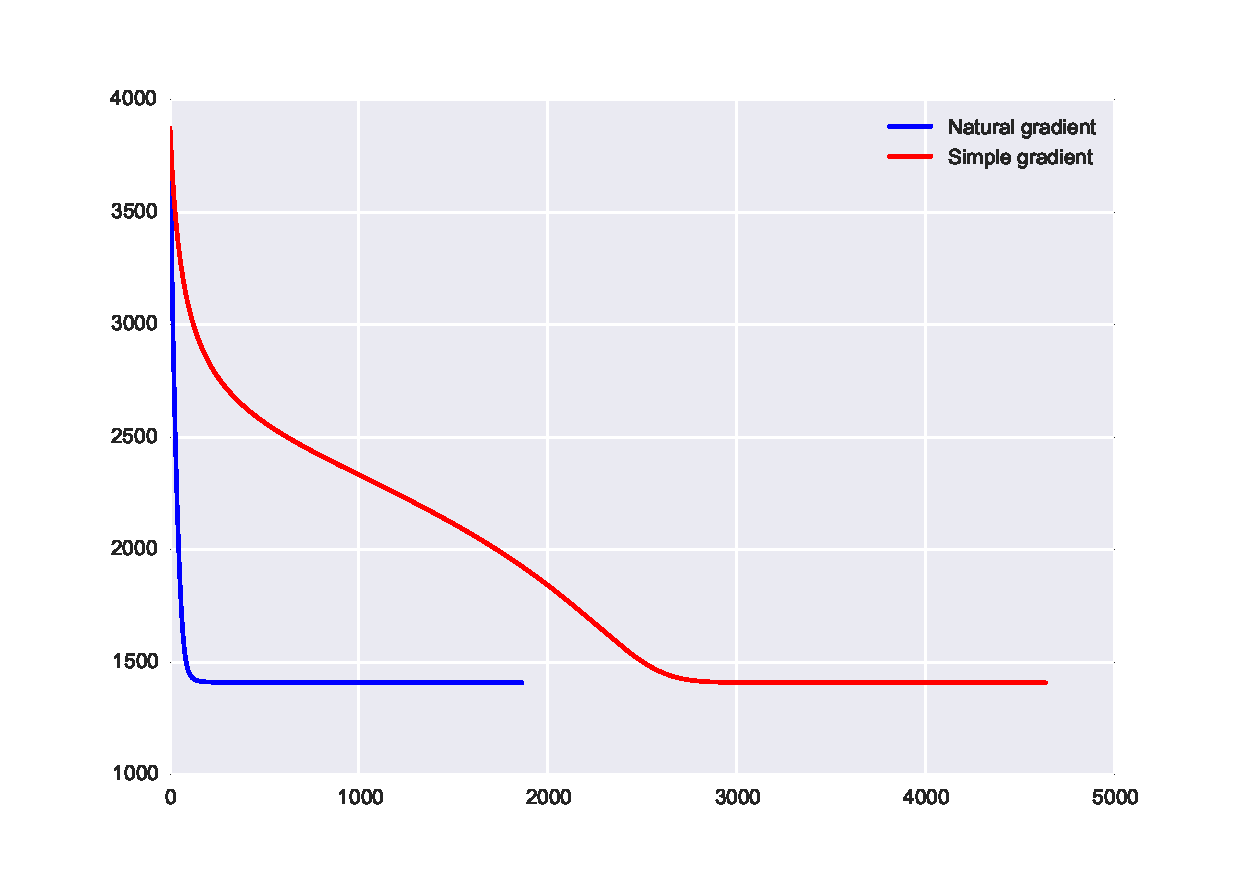
\includegraphics[scale=0.8, trim=1.5cm 0 0 0]{figure_5}
        \end{flushleft}

        \newpage

        Точки по которым проходили методы стандартного и натурального градиента:
        \begin{flushleft}
            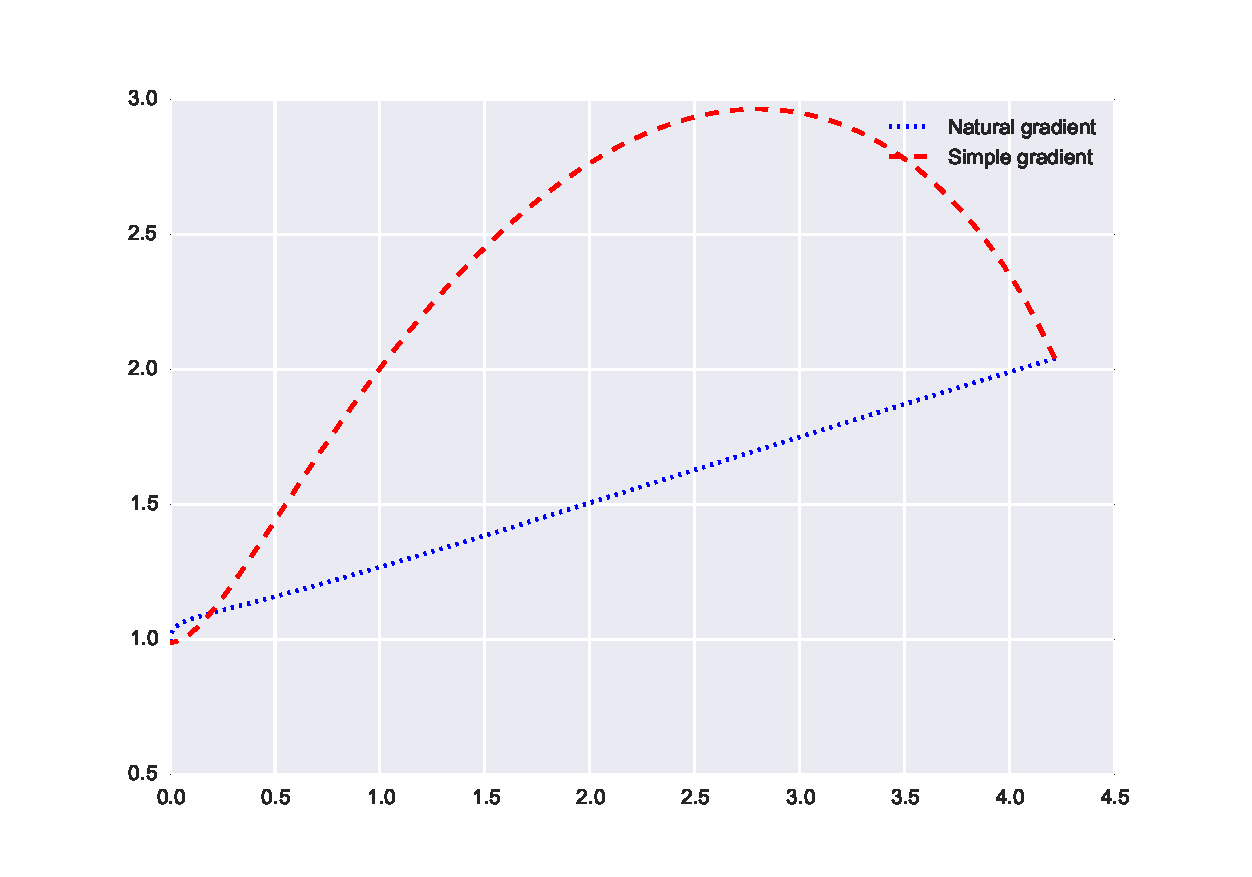
\includegraphics[scale=0.8, trim=1.5cm 0 0 0]{figure_55}
        \end{flushleft}

        Видно, что метод натурального градиента практически сразу сошелся к нужному значению параметров распределения.
        Также, метод натурального градиента сразу выбрал правильное направление на плоскости параметров $(a, \sigma)$, 
        в отличие от метода стандартного градиентного спуска.

\newpage

\subsection{Полярная система координат}
\subsubsection{Описание}
        Рассмотрим другой пример: дана функция $f(r, \phi) = (r ~ cos \phi -1)^2 + (r ~ sin \phi)^2$.
        Ясно, что если мы перейдем к замене
        $$
            \begin{aligned}
                & x = r cos \phi \\
                & y = r sin \phi
            \end{aligned},
        $$
        то получим функцию $g(x, y) = (x - 1)^2 + y^2$. Ее минимум находится в точке $(x,~ y) = (1,~ 0)$. Однако из-за
        перехода в исходной функции к полярной системе координат стандартный градиентный спуск работает несколько иначе и не находит прямой путь в минимум.
        Найдем градиент:
        $$
            \nabla f(r, \phi) = 
            \left[
                \begin{aligned}
                    & 2(r - cos \phi) \\
                    & 2r sin \phi
                \end{aligned}
            \right]
        $$
        
        Метрический тензор Римана для полярных координат был найден на стр. \pageref{PolarTensor}.
        \newpage

\subsubsection{Результаты и графики}

        В качестве начальных значений параметров выбирались случайные начальные значение от 0 до 10 и от 0 до $2\pi$ для $r$ и $\phi$ соответственно.
        Параметры алгоритмов:
        $$
            \begin{aligned}
                & \alpha = 0.01 \\
                & \varepsilon = 0.0001
            \end{aligned}
        $$

        Зависимость значения функции от числа итераций:
        \begin{flushleft}
            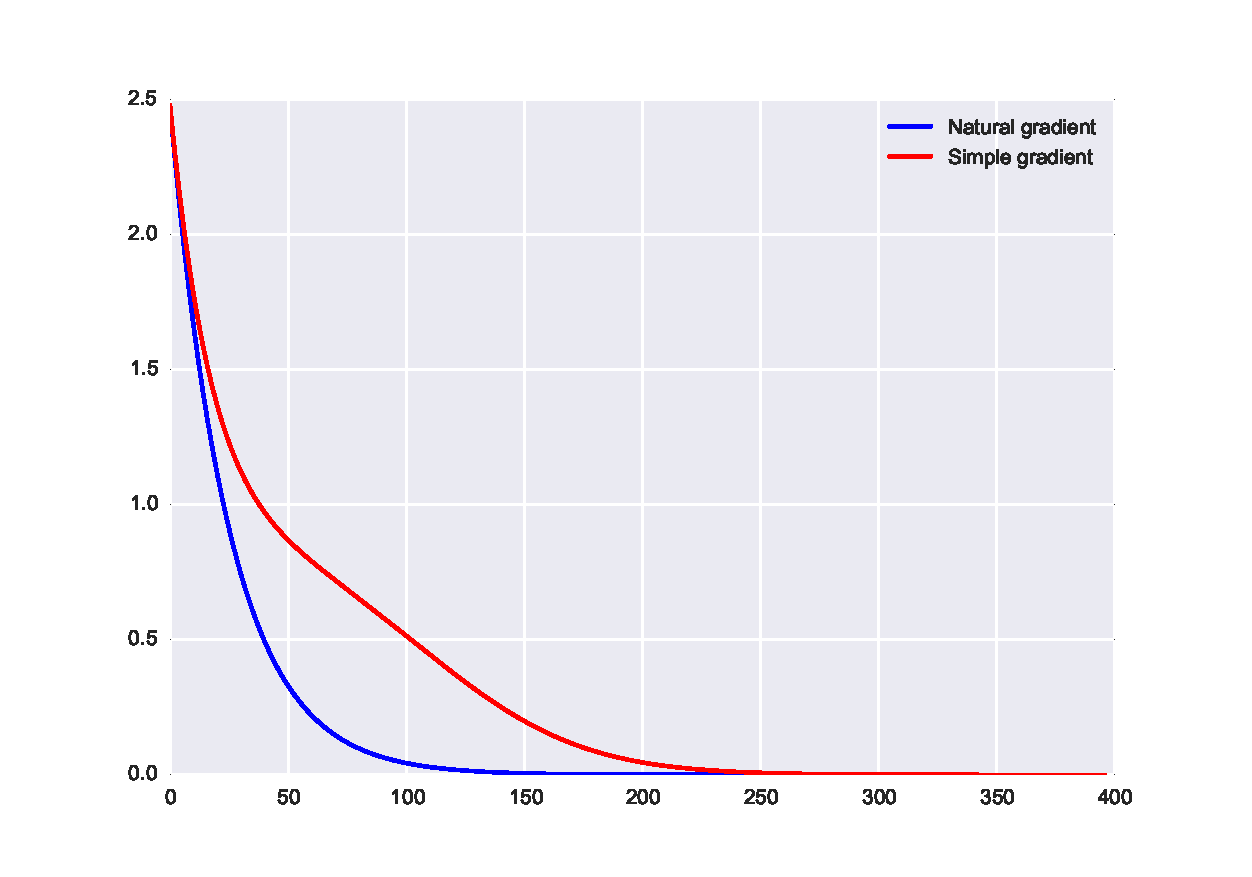
\includegraphics[scale=0.8, trim=1.5cm 0 0 0]{figure_6}
        \end{flushleft}

        \newpage

        Точки по которым проходили методы стандартного и натурального градиента:
        \begin{flushleft}
            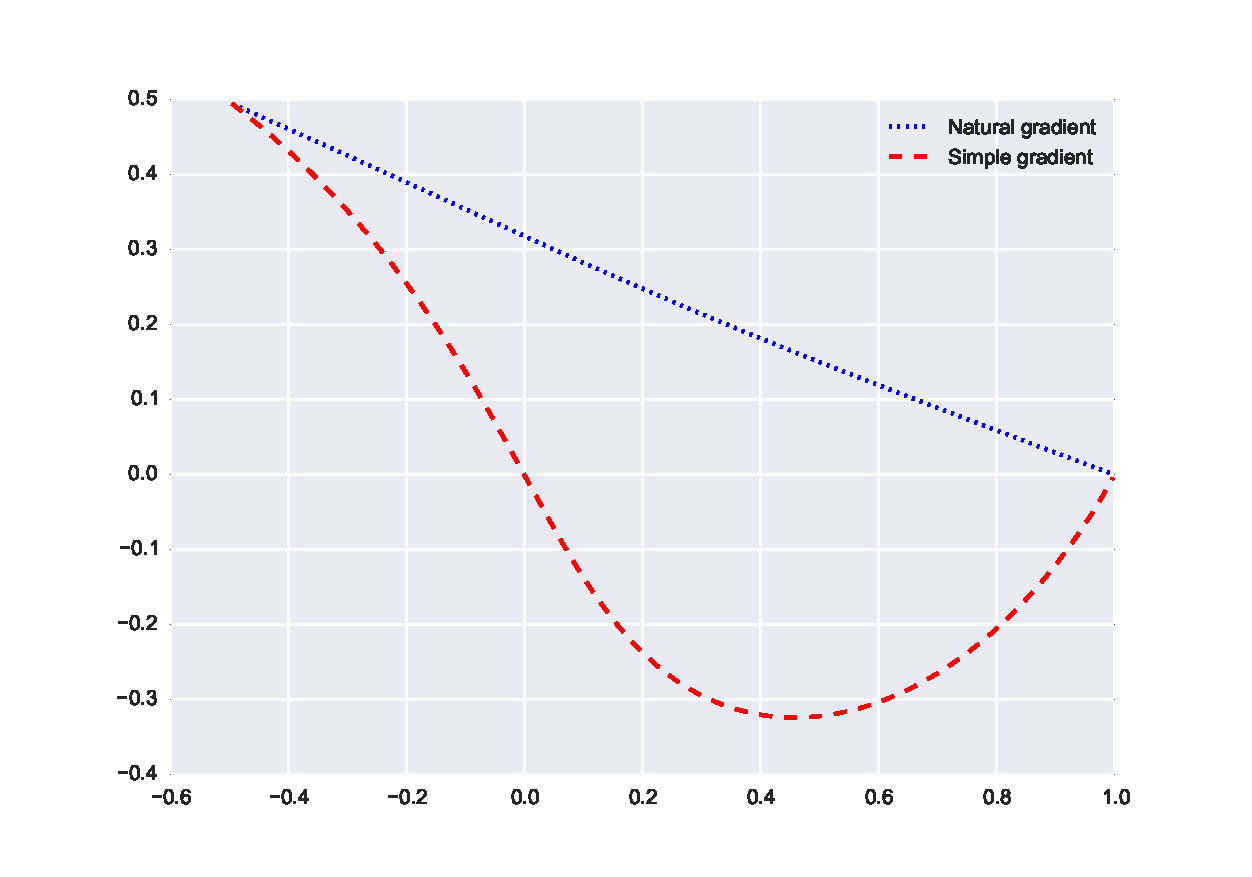
\includegraphics[scale=0.8, trim=1.5cm 0 0 0]{figure_66}
        \end{flushleft}

        В данном примере метод натурального градиента примерно в 2 раза быстрее сошелся к минимуму.
        Метод натурального градиента снова сразу выбрал правильное направление на плоскости параметров $(r, \phi)$, 
        в отличие от метода стандартного градиентного спуска.

\newpage

\section{Применения натурального градиента}
\begin{enumerate}
    \item Обучение нейронных сетей

        Нейронные сети являются широким разделом алгоритмов машинного обучения.
        Их необходимо обучать подбирая некоторые параметры --- веса. Подбор осуществляется методом градиентного спуска.
        Этот метод можно улучшить применяя метод натурального градиента.

    \item Слепое разделение источников сигнала

        Данная задача подразумевает, что мы знаем, что есть несколько источников сигнала, и что эти сигналы могут смешиваться
        друг с другом. Однако мы не знаем каким именно образом они смешиваются и задача состоит в том, чтобы разделить их.

    \item Слепая развертка сигналов

        Эта задача похожа по формулировке на предыдущую, однако, отличается от нее тем фактом, что текущие сигналы могут смешиваться
        с предыдущими. Тут также используется метод натурального градиента.

    \emph{Примечание}:
        Применение натурального градиента для решения вышеописанных проблем описаны в \cite{AmariWorks}
\end{enumerate}
\newpage
 
\section{Заключение}
Метод натурального градиента имеет свои преимущества над другими методами оптимизации. Он позволяет находить естественное для пространства параметров направление наискорейшего спуска. Однако он не лишен недостатков: 
\begin{enumerate}
    \item Необходимо глубокое понимание проблемы для нахождения $G(w)$. 
    \item Обращение матрицы --- вычислительно довольно затратная операция. В целом, метод натурального градиента часто сходится быстрее остальных.
\end{enumerate}
\newpage 

\section{Список литературы}
\nocite{*}
\printbibliography[heading=none]
\newpage

\section{Приложение}

Реализация натурального градиента.
%\lstinputlisting[language=Python]{code/natgrad.py}
\inputminted{python}{code/natgrad.py}
\newpage
Тест с нормальным распределением.
%\lstinputlisting[language=Python]{code/likelihood_test.py}
\inputminted{python}{code/likelihood_test.py}
\newpage
Тест с полярной системой координат.
%\lstinputlisting[language=Python]{code/polar_test.py}
\inputminted{python}{code/polar_test.py}
\newpage
Основной файл.
%\lstinputlisting[language=Python]{code/main.py}
\inputminted{python}{code/main.py}
\newpage

\end{document}
